%\documentclass{jarticle}
%\newcommand{\figref}[1]{\figurename\ref{#1}}
%\newcommand{\tabref}[1]{\tablename\ref{#1}}
%\usepackage[dvipdfmx]{graphicx}
%\begin{document}

%\section{解析}
% この部分にエネルギー解析のみの記載しかしておらず時間解析に関する記述が必要?
\subsection{エネルギー解析}
信号解析で求められたエネルギー値を元にエネルギースペクトルを求め,それを元にミッシェルパラメータを求めるための各種解析を行った.まずは各種時間情報を元にスピンの向きに関する考察をし,さらにバックグラウンドの影響を考えてイベントのセレクションを行った.また,エネルギースペクトルに対するフィッティングでは検出器内での電磁シャワーによるエネルギー応答を考慮して行列を関数に畳み込んで最小二乗法を適用した.

\subsubsection{スピンの回転に関して}
当初の目標に反して$g$ 因子測定用に用意した磁場をかけた標的を用いて測定したデータを用いて以下の解析を行った.大きな要因としてはこのデータを元に解析を行っても解析ができることがわかったため,長い時間を測定しイベント量を多く採れたデータを使う方が統計誤差の観点から良いと考えたからである.また,このデータではいろいろな方向のスピン方向の情報を持っているため,スピンに関わるミッシェルパラメータである$\xi,\delta$ の測定も可能である.以下ではまず時間情報を元にスピン方向のデータが求められる事をみる.

時間に関してヒストグラムを出すと$g$ 因子の解析で出たような指数関数と三角関数の積の形で出てくる.このままでは例えば$\rho$ を求めるためのスピン無偏極のデータを得るためにスピン全方向に対応する一周期分の時間範囲のデータを取り出しても,指数関数分の減衰があるため,後ろの時間のスピン情報が軽視されスピン方向を等価に足しあわせられず完全にキャンセルすることができない.これは指数関数の減衰の影響によるものなので,逆にその逆数で重みをつけてやることでその影響をキャンセルできることを確認する.ここではミューオンの崩壊寿命$\tau=2.2\mu \mathrm{s}$ を既知としてそれぞれのデータに関して$\exp(t/\tau)$の重み付けを行った.すると時間情報のヒストグラムは\figref{hatano_fig:oscillation} となった.これは実際に指数関数の影響をキャンセルして,スピンに由来する情報のみを取り出せてることを示している.改めて確認するとスピンの向きは三角関数の最大値が$\theta=0$,最小値が$\theta=\pi$ に対応する.

\begin{figure}[hbt]
\centering
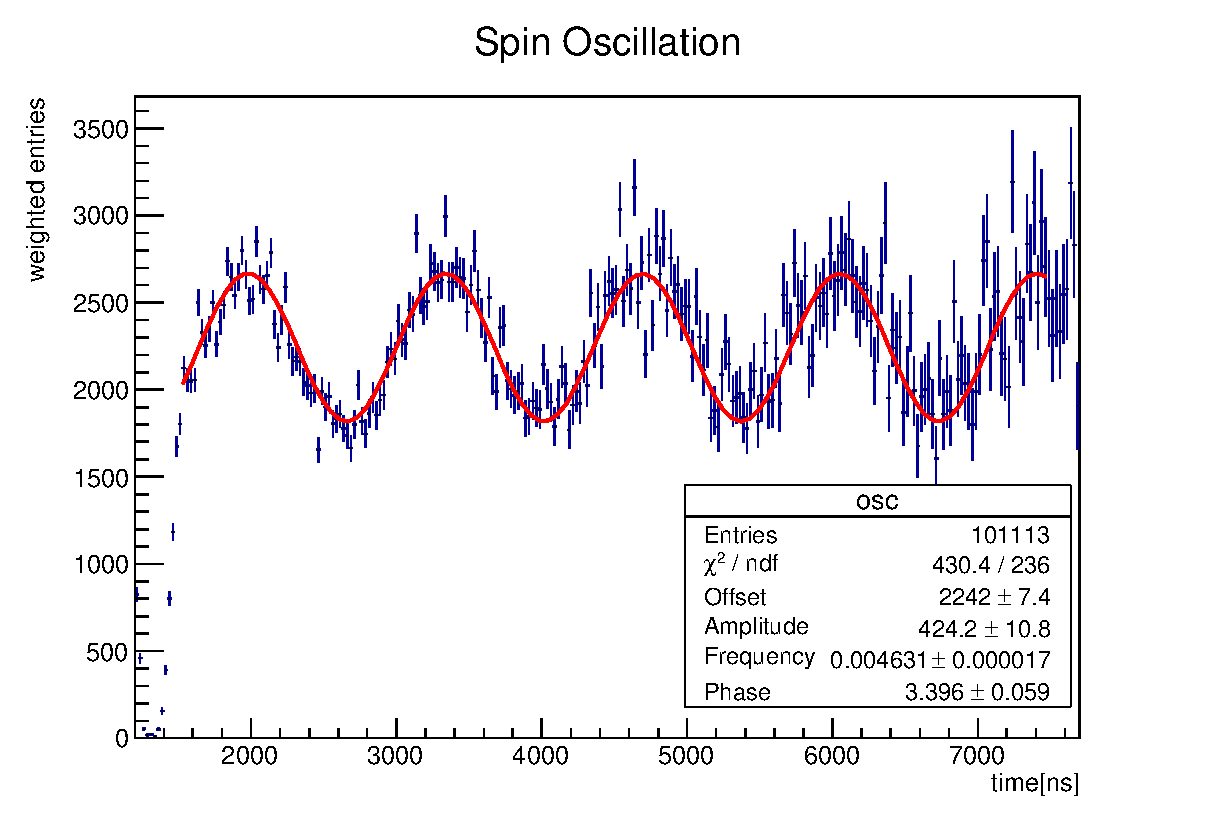
\includegraphics[width=0.8\textwidth]{figure/hatano/oscillation.eps}
\caption{時間に対するスピンによる計数の変動の様子}
\label{hatano_fig:oscillation}
\end{figure}

以上より,同様の重み付けをした上で適切な時間範囲をとることで任意のスピンの向きに関するエネルギースペクトルを取り出すことができる.

\subsubsection{イベントセレクション}
今回の測定データでは各NaI チャンネル毎のデータがあるため,位置によるエネルギーの違いに基づいてバックグラウンドのデータを減らすためにイベントをセレクションした.具体的には概ね標的方向からの粒子は中心のNaI にエネルギーを落とすと考えられるので,中心のNaI と全体とのエネルギー比によってイベントセレクションをした.いろいろな割合で試したのが\figref{hatano_fig:bg}である.あまり,中心にエネルギーが入ってきたという制約を加えるとそれ以上割合を動かしてもイベント数が減るだけで相対的な形は大きく変動がなく以下の解析でも大きな変化はなかったため,今回は中心に全体の半分以上のエネルギーが入っているという制約を加えた.

\begin{figure}[hbt]
\centering
\includegraphics[width=0.8\textwidth]{figure/hatano/bg.eps}
\caption{イベントカットによる変動}
\label{hatano_fig:bg}
\end{figure}

\subsubsection{検出器の電磁シャワー応答について}
今回の検出器は全吸収型のカロリメータではあるが,検出器内で形成された電磁シャワーで主に$\gamma$ 線となったものが検出器内から漏れる事が多いため,必ずしも入射した粒子のエネルギーに対応する形でエネルギーが測定されるわけではなく,低エネルギーの裾をもつ確率分布でエネルギーが与えられる.ただし,この関数形を解析的な形で求めることは難しいので今回はシミュレーション(Geant4)を行って,それらの応答を計算した.結果は\figref{hatano_fig:response}となった.

\begin{figure}[hbt]
\centering
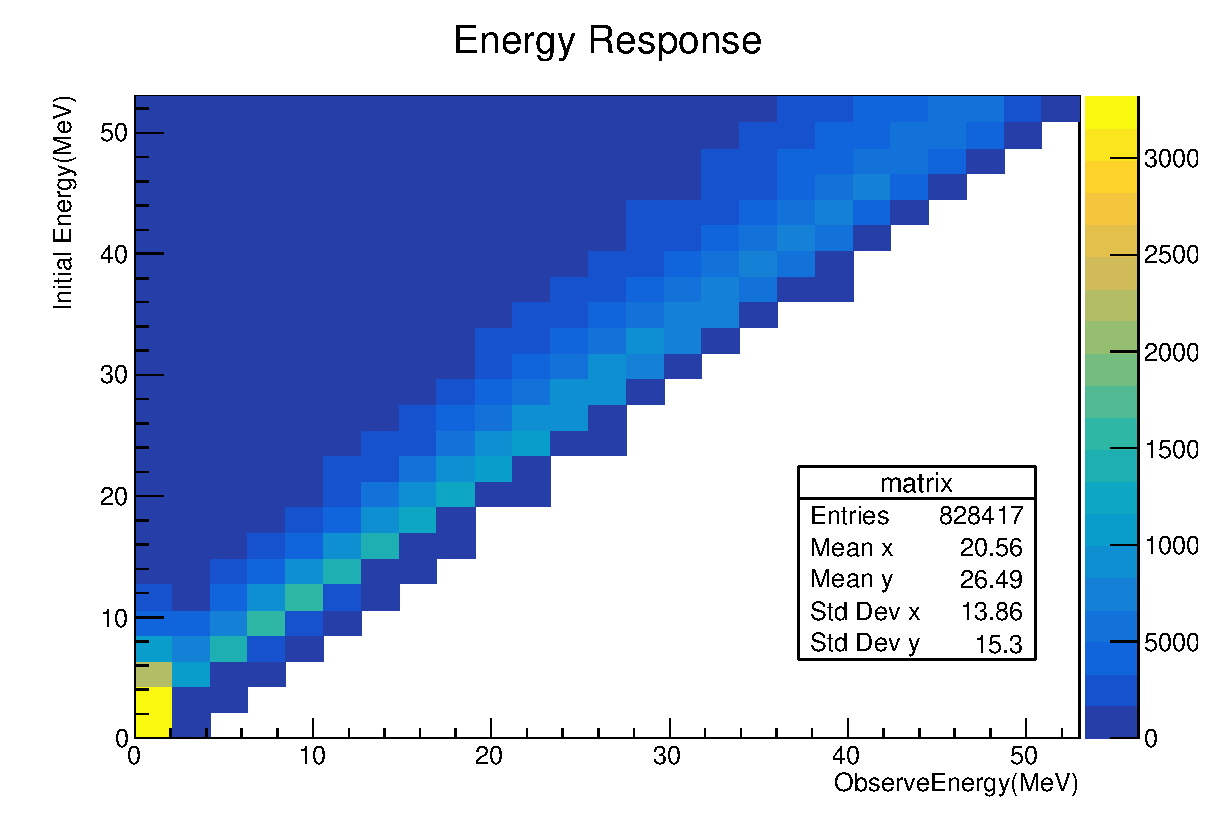
\includegraphics[width=0.8\textwidth]{figure/hatano/response.eps}
\caption{カロリメータ内の電磁シャワー応答}
\label{hatano_fig:response}
\end{figure}

以下フィッティングの際にはこの応答を畳み込んだ最小二乗法を用いた.最小二乗法については付録に掲載する.

\subsubsection{ミッシェルパラメータ$\rho$の導出}
スピンを全範囲で積分して無偏極とすれば,エネルギースペクトルは$f(x)=(3 - 3x / E_\mathrm{max})+\frac{2}{3}\rho(4x - E_\mathrm{max} - 3)$ として表される.ここでは,無偏極データを得るために\figref{hatano_fig:response}の最初の三周期に相当する時間範囲を重みづけて抽出した.

このフィッティングは高エネルギー部分の変動に対して極めて鋭敏であり,そのため較正係数の誤差に対して極めて鋭敏である.一方で今回の測定では較正の精度があまりよくなく大きな系統誤差を与えると考えられる.ここでは較正係数を測定から想定される$\pm 20~\%$ の範囲で動かし,最も適当な当てはめができたとき($\chi^2$ が最小なとき)を測定値とした.フィッティングの結果は\figref{hatano_fig:rho} である(バックグラウンド項として一次関数$p_2+p_3x$を仮定した).この時のフィッティングのパラメータは$p_0(3 - 3x / E_\mathrm{max}) + \frac{2}{3} p_{1} (4x / E_\mathrm{max} - 3)$ と書くと,\tabref{hatano_tab:rho} となった.これより,$\rho=0.663 \pm 0.023$ となった.
\begin{table}[hbt]
\centering
\caption{$\rho$ のフィッティングパラメータ}
\begin{tabular}{cccccccc}
$p_0$ & $\delta p_0$ & $p_1$ & $\delta p_1$ & $p_2$ & $\delta p_2$ & $p_3$ & $\delta p_3$ \\ \hline
3.092 & 0.011 & 4.665 & 0.128 & 1476.440 & 0.158 & -2.660 & 0.011
\end{tabular}
\label{hatano_tab:rho}
\end{table}

また,フィッティングパラメータが$1\sigma$ ずれると$\chi^{2}+1$ となるため$\chi^{2} + 1$ の範囲を系統誤差とした.最大で0.801,最小で0.617 であり最大幅である0.138 を系統誤差とした.以上の結果をまとめると$\rho=0.663 \pm 0.023 \pm 0.138$ である.

\begin{figure}[hbt]
\centering
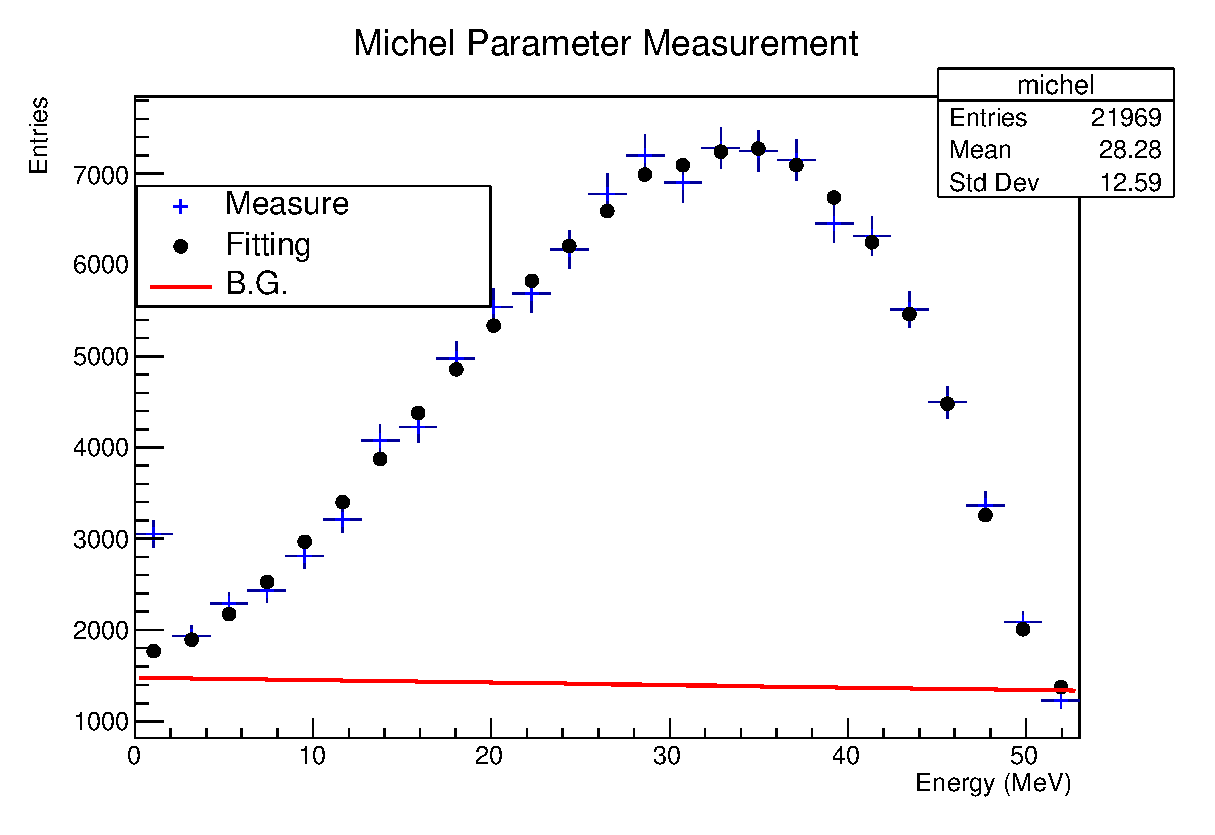
\includegraphics[width=0.8\textwidth]{figure/hatano/rho.eps}
\caption{$\rho$ のフィッティングの様子}
\label{hatano_fig:rho}
\end{figure}

\subsubsection{ミッシェルパラメータ$xi$ の導出}
スピンに対する計数の変化を考えると計数はビームが100~\%偏極$P_{\mu} = 1$なので$dN / d \cos \theta \propto 1 + \frac{1}{3} \xi \cos \theta$ となる.これを用いてミッシェルパラメータ$\xi$ を求める.
スピンが手前を向いているとき ($0\leq\theta\leq\frac{\pi}{2}$) の計数$N_+$ と逆を向いているとき ($\frac{\pi}{2}\leq\theta\leq\pi$) の計数$N_-$ の比を見ると,$N_{+} / N_{-} =  (6 + \xi) / (6 -\xi)$であるのでこれを求めればよい.これらはスピンの向きに関する部分の測定なので,単純なバックグラウンドだけでなくターゲット内散乱により無偏極となったものによるバックグラウンドも考えなければならない.特に後者の影響を見積もる事は難しいが,どちらも$\xi$ を小さく見積もる方向に影響を与える.

最初の一周期の該当する範囲で計数を考えると$N_+=73607.5$,$N_-=52878.6$ となる.ここでも,指数関数の重みをつけていることを忘れてはいけない.以上より,この比を$R=N_{+} / N_{-}$ とすると$\xi=6\frac{R-1}{R+1}$ より求まり,$\xi=0.983\pm0.017$ となる.

\subsubsection{ミッシェルパラメータ$\delta$ の導出}
スピンがある方向を向いている時のスペクトルを見ることにより,残るミッシェルパラメータの$\delta$ を含む形で表される.ただし,あるスピンを適当に選び抜き$\delta$ を測定するには$\rho$ や$\xi$ などのパラメータを含む形になりパラメータの数が多くなる.ここで,ちょうどスピンが反対のものを差し引くと$\rho$ の関わる部分がキャンセルをし,$\xi$ は比例係数の内に含まれるため,$\delta$ のみでエネルギースペクトラムは表され,$(1-\frac{x}{E_{max}})+\frac{2}{3}\delta(4\frac{x}{E_{max}}-3)$という形の関数で表される.

実際にはスピンが手前を向いているとき ($0\leq\theta\leq\frac{\pi}{2}$) と逆を向いているとき ($\frac{\pi}{2}\leq\theta\leq\pi$) を差し引いたスペクトルに対して$\rho$ の解析と同様にフィッティングを行った.$\rho$ の導出と同様に較正係数を動かして適切なフィッティングを決めた.その様子が\figref{hatano_fig:delta} である.またその結果が\tabref{hatano_tab:delta} であり,$\delta=0.613\pm0.112$ である.また系統誤差は最小で0.464,最大で0.794 となったので最大幅の0.181 とした.すなわち$\delta=0.613\pm0.112\pm0.181$ である.
\begin{table}[hbt]
\centering
\caption{$\delta$のフィッティングパラメータ}
\begin{tabular}{cccccccc}
$p_0$ & $\delta p_0$ & $p_1$ & $\delta p_1$ & $p_2$ & $\delta p_2$ & $p_3$ & $\delta p_3$ \\ \hline
0.978 & 0.123 & 1.595 & 0.211 & 104.741 & 2.722 & 0.211 & 0.123 \\
\end{tabular}
\label{hatano_tab:delta}
\end{table}

\begin{figure}[hbt]
\centering
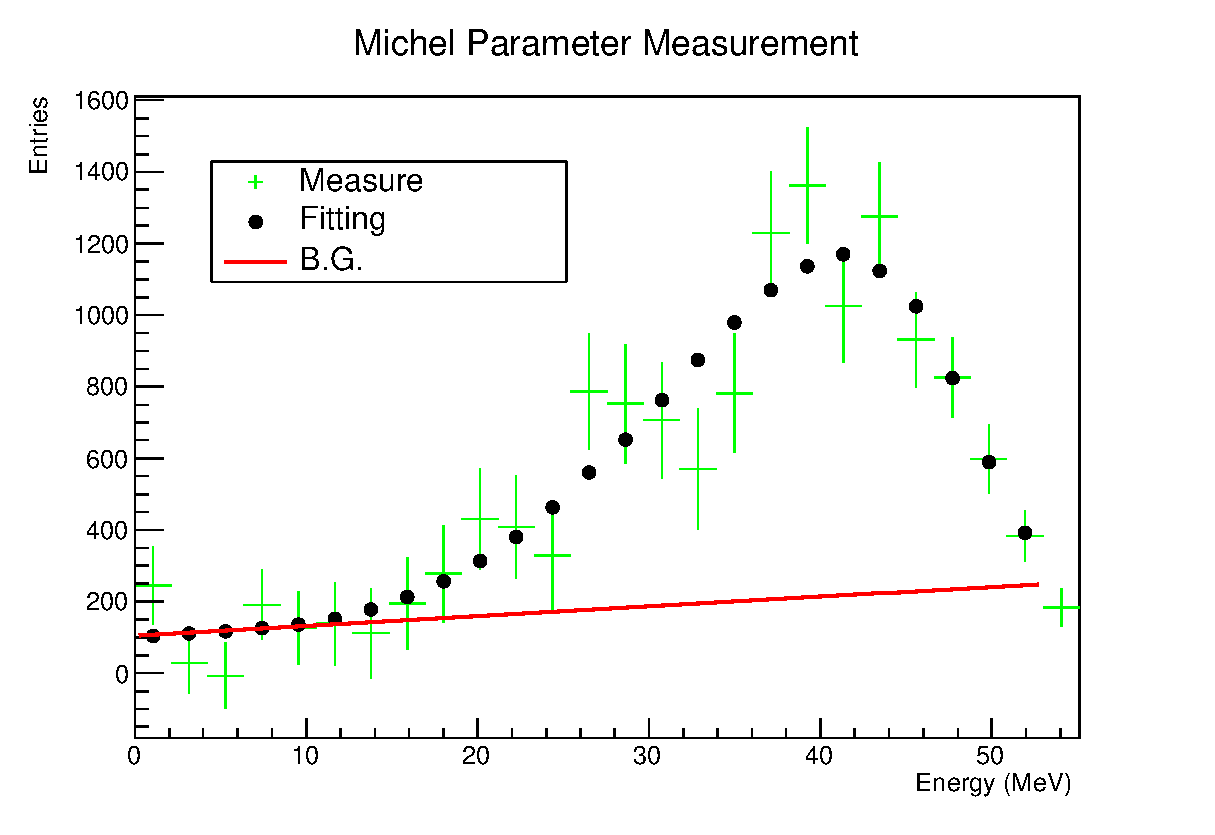
\includegraphics[width=0.8\textwidth]{figure/hatano/delta.eps}
\caption{$\delta$ のフィッティングの様子}
\label{hatano_fig:delta}
\end{figure}

%\end{document}
